\section{Результаты работы}
В качестве метрик качества выбраны стандартные метрики для регрессии --- среднеквадратичная и средняя абсолютная ошибки, а также максимальная ошибка и коэффициент детерминации $R^2$.

В отличие от случайного леса, которому необходимы деревья максимальной глубины, градиентному бустингу нужны не переобученные деревья. Поэтому сначала определим оптимальные гиперпараметры одиночного дерева при помощи кросс-валидации.

Оптимальная глубина дерева: 20, минимальный размер листа: 5, критерий построения дерева: среднеквадратичная ошибка, способ вычисления ответа: среднее значение.

Одиночное дерево показывает следующие результаты:
\begin{lstlisting}[frame=none, numbers=none]
Max error: 41.984262068
MAE: 5.772610978436216
MSE: 73.80822161902006
R^2: 0.7168804103896775
\end{lstlisting}
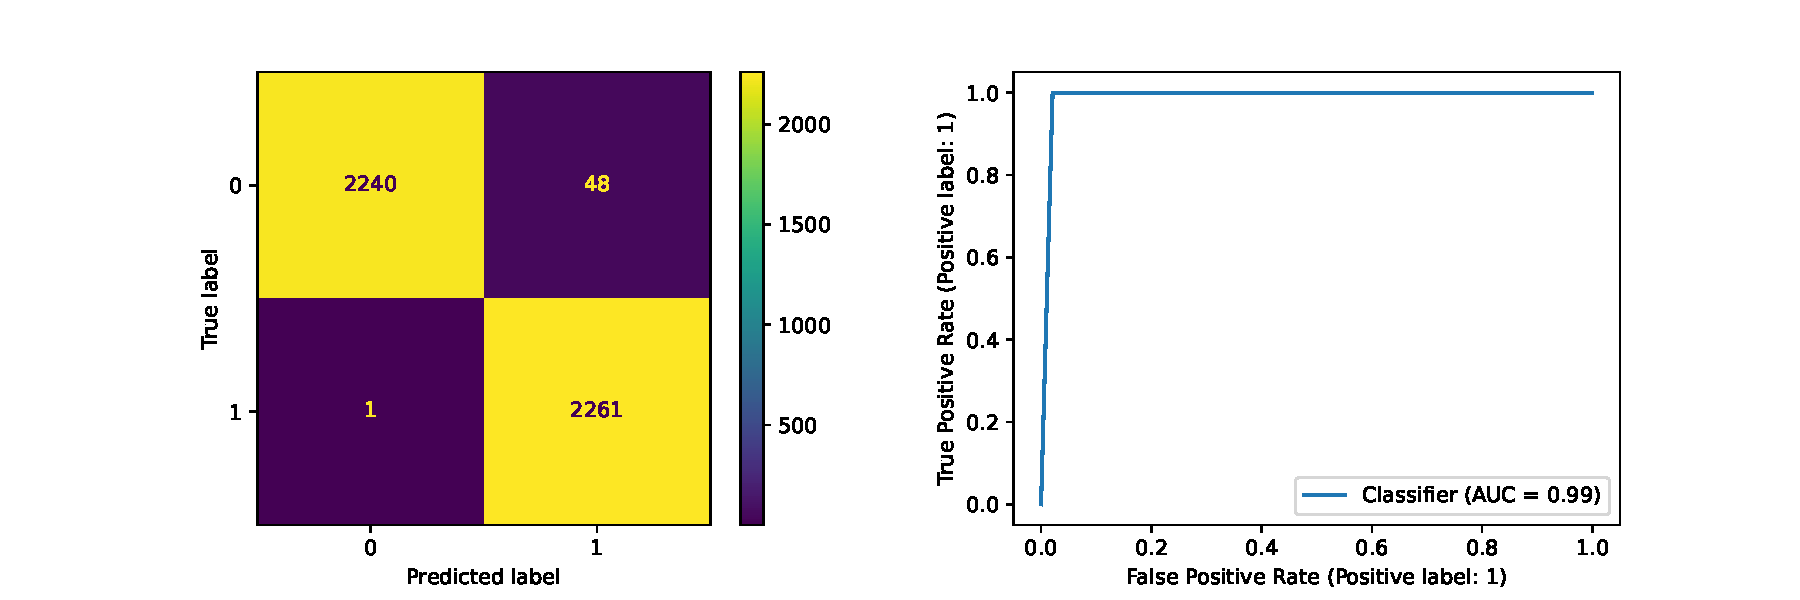
\includegraphics[scale=0.63]{tree}

\pagebreak
Сравним его с деревом из sklearn с теми же параметрами:
\begin{lstlisting}[frame=none, numbers=none]
Max error: 46.51205096
MAE: 5.184229691927071
MSE: 67.95003686449105
R^2: 0.7393517127348934
\end{lstlisting}
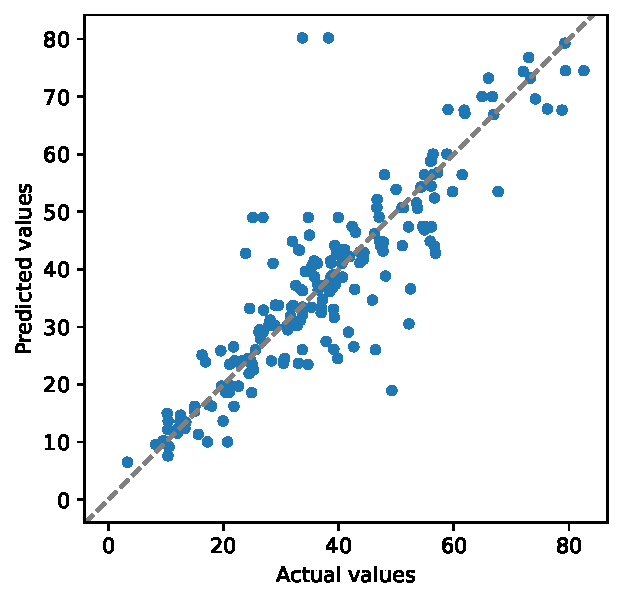
\includegraphics[scale=0.63]{sk_tree}

Результаты довольно похожи.

Будем использовать получившиеся параметры дерева для градиентного бустинга, гиперпараметры же самого бустинга снова определим через кросс-валидацию.

Оптимальное число деревьев: 80, скорость обучения: 0.1.

Градиентный бустинг показывает следующие результаты:
\begin{lstlisting}[frame=none, numbers=none]
Max error: 31.724549658115357
MAE: 4.5016877121038945
MSE: 50.426762544929396
R^2: 0.8065689159834937
\end{lstlisting}
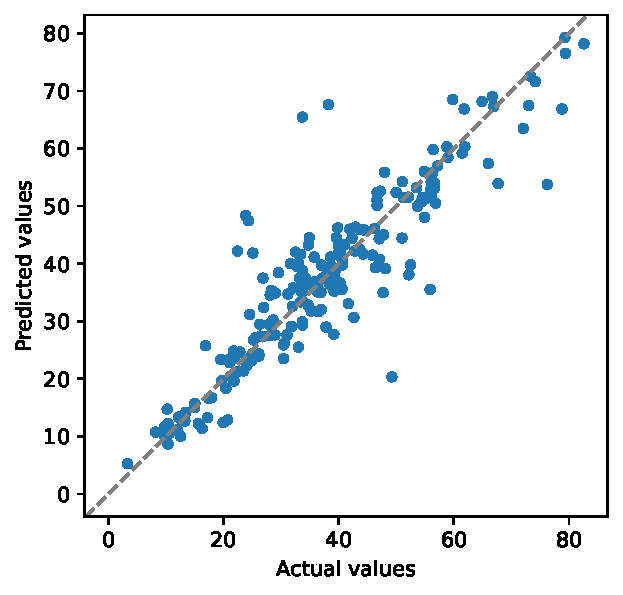
\includegraphics[scale=0.63]{gb}

\pagebreak
Сравним с градиентным бустингом из sklearn с теми же параметрами:
\begin{lstlisting}[frame=none, numbers=none]
Max error: 31.774143301871298
MAE: 4.478631496353804
MSE: 48.81379503539908
R^2: 0.8127560681643196
\end{lstlisting}
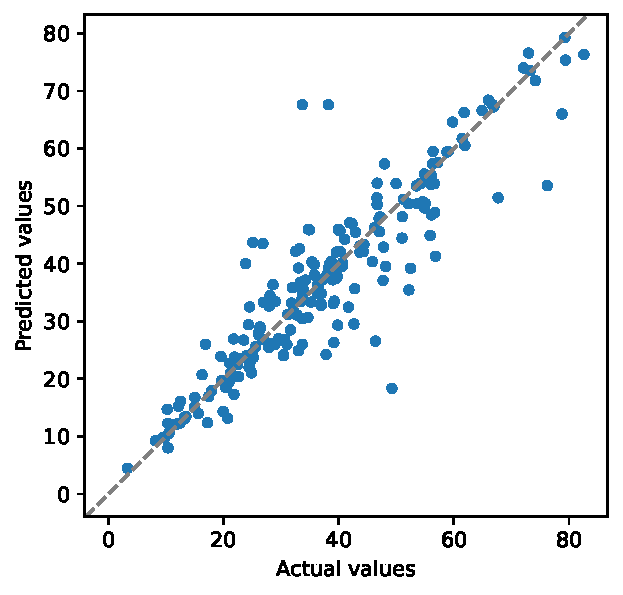
\includegraphics[scale=0.63]{sk_gb}

Результаты очень похожи, разница в ошибках порядка десятых, $R^2$ отличается меньше чем на 0.01. 

\pagebreak

